
\section{Lý thuyết Bass-Serre}
Lý thuyết Bass-Serre là một công cụ giúp ta nghiên cứu nhóm thông qua tác động chúng lên cây. Cụ thể, thông qua tác động, ta có thể phân tích nhóm thành tích amalgam của các nhóm con. Trong phần này tôi sẽ trình bày lại một phần của lý thuyết trên, nội dung tham khảo chủ yếu từ \cite{TreeSerre}.

\subsection{Tích amalgam}
Định nghĩa cho tích amalgam phụ thuộc vào định nghĩa giới hạn trực tiếp (\ref{def:direct-limit}) trên phạm trù \textbf{Grp}. Nếu ta xét phạm trù tổng quát thì giới hạn không phải lúc nào cũng tồn tại, tuy nhiên trong phạm trù \textbf{Grp} thì giới hạn luôn tồn tại dựa trên một cách xây dựng cụ thể:

\begin{proposition}[\cite{TreeSerre}]\label{prop:unique_direct_limit}
    Cho $\{G_i\}_{i \in I}$ là một họ các nhóm và $F_{ij} \subset \Hom(G_i, G_j)$ với mỗi $(i,j) \in I \times I$. Giới hạn trực tiếp của hệ $(G_i,F_{ij})$ tồn tại duy nhất sai khác một đẳng cấu.
\end{proposition}

\startproof Tính duy nhất được suy ra từ tính phổ dụng của giới hạn trực tiếp. Về sự tồn tại, ta có thể xét nhóm tự do sinh bởi $\bigsqcup G_i$ chia cho quan hệ
\begin{itemize}
    \item $z=xy$ nếu $x,y,z \in G_i$ và $z=xy$ trong $G_i$.
    \item $x=y$ nếu $x \in G_i, y\in G_j$ và $y=f(x)$ với $f \in F_{ij}$ nào đó.\qed
\end{itemize}

\begin{define}[\cite{TreeSerre}]
    Xét các nhóm $A,G_1,G_2$ và các đồng cấu $f_1: A \rightarrow G_1, f_2: A \rightarrow G_2$. Giới hạn trực tiếp của hệ trên được gọi là \textdef{tích amalgam} của $G_1$ và $G_2$ trên $A$ thông qua $f_1$ và $f_2$, kí hiệu $G_1 *_A G_2$.
    $$
        \begin{tikzcd}
            A \arrow[d, "f_2"'] \arrow[r, "f_1"] & G_1 \arrow[d] \\
            G_2 \arrow[r]                        & G_1 *_A G_2
        \end{tikzcd}
    $$
\end{define}

Từ \ref{prop:unique_direct_limit} ta có một biểu diễn cụ thể cho tích amalgam
$$
    G_1 *_A G_2 = \langle S_1, S_2\ |\ R_1, R_2,\ f_1(a) = f_2(a),\ \forall a \in A \rangle
$$
trong đó $G_1 = \langle S_1\ |\ R_1 \rangle, G_2 = \langle S_2\ |\ R_2 \rangle$.

\begin{define}
    \textdef{Tích tự do} $G_1 * G_2$ giữa hai nhóm $G_1$ và $G_2$ là tích amalgam của $G_1$ và $G_2$ trên nhóm tầm thường.
\end{define}

\subsection{Cây}
\begin{define}[\cite{TreeSerre}]
    Một \textdef{đồ thị} $\Gamma$ bao gồm tập các đỉnh $V = \ver \Gamma$, tập các cạnh $E = \edge \Gamma$ và hai ánh xạ
    \begin{align*}
         & E \rightarrow  V \times V  & E \rightarrow  E            \\
         & e \mapsto      (o(e),t(e)) & e \mapsto      \overline{e}
    \end{align*}
    thỏa $\overline{\overline{e}} = e$, $\overline{e} \neq e$ và $o(e) = t(\overline{e})$. Khi đó ta gọi $o(e)$, $t(e)$ và $\overline{e}$ lần lượt là \textdef{đỉnh đầu}, \textdef{đỉnh cuối} và \textdef{nghịch đảo} của cạnh $e$.
\end{define}

\begin{define}[\cite{TreeSerre}]
    Một \textdef{định hướng} của đồ thị $\Gamma$ là tập con $E_+$ của $E = \edge \Gamma$ sao cho $E = E_+ \bigsqcup \overline{E_+}$. Một \textdef{đồ thị có hướng} gồm tập các đỉnh $X$, tập các cạnh $E_+$ và ánh xạ $E_+ \rightarrow V \times V$.
\end{define}

\begin{define}[\cite{TreeSerre}]
    Một \textdef{cấu xạ} giữa hai đồ thị $\Gamma$ và $\Gamma'$ là cặp các ánh xạ
    $$
        \alpha: \ver \Gamma \rightarrow \ver\Gamma'\quad\text{và}\quad \beta: \edge \Gamma \rightarrow \Gamma'
    $$
    thỏa $\alpha(o(y)) = o(\beta(y))$ và $\overline{\beta(y)} = \beta(\overline{y})$. Cấu xạ giữa hai đồ thị được gọi là \textdef{đẳng cấu} nếu $\alpha$ và $\beta$ là song ánh. Tập tất cả các đẳng cấu từ đồ thị $\Gamma$ vào chính nó được kí hiệu là $\Aut(\Gamma)$.
\end{define}

\begin{define}[\cite{TreeSerre}]
    Cho $\Gamma$ là đồ thị với $V = \ver \Gamma,\ E = \edge \Gamma$. Ta xét không gian tôpô $T = V \bigsqcup (E \times [0,1])$, trong đó $V$ và $E$ được trang bị tôpô rời rạc. Gọi $R$ là quan hệ tương đương trên $T$ cho bởi $(e,t) \equiv (\overline{e}, 1-t)$, $(e,0) \equiv o(e)$ và $(e,1) \equiv t(e)$ với $e \in E,\ t \in [0,1]$. Khi đó không gian thương $\real \Gamma = T/R$ được gọi là một \textdef{nhận dạng} của đồ thị $\Gamma$.
\end{define}

\begin{define}[\cite{TreeSerre}]
    Cho $n$ là số nguyên $\geq 0$. Xét đồ thị có hướng
    \begin{figure}[H]
        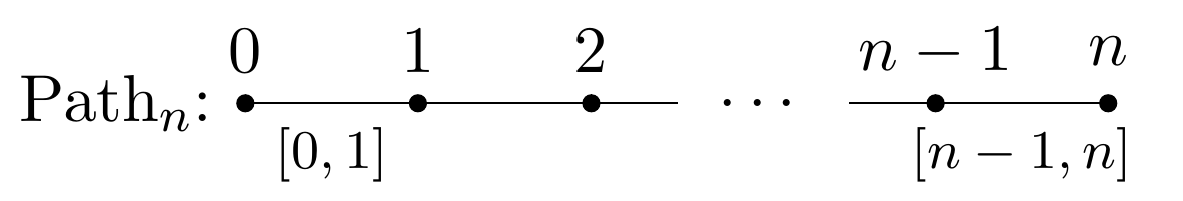
\includegraphics[width=8cm]{assets/path-graph.png}
        \centering
    \end{figure}
    trong đó $\{0,1,...,n\}$ là các đỉnh của đồ thị, $\{[i,i+1] \mid 0 \leq i < n \}$ là các cạnh của đồ thị, với định hướng được xác định bởi $o([i,i+1]) = i$ và $t([i,i+1]) = i+1$.
\end{define}

\begin{define}[\cite{TreeSerre}]
    Một \textdef{đường đi (với chiều dài $n$)} của đồ thị $\Gamma$ là một cấu xạ từ $c: \Path_n \rightarrow \Gamma$.

    Dãy các cạnh $(y_1,...,y_n)$ với $y_i = c([i-1,i])$ sao cho $t(y_i) = o(y_{i+1})$ xác định đường đi $c$. Nếu $P_i = c(i)$ thì ta nói $c$ là đường đi từ $P_0$ đến $P_n$ và ta gọi chung $P_0, P_n$ là các \textdef{đỉnh đầu cuối}.

    Một cặp cạnh có dạng $(y_i,y_{i+1}) = (y_i,\overline{y_i})$ trong đường đi được gọi là \textdef{quay lui}. Bằng cách loại bỏ đi một quay lui, ta có thể xây dựng đường đi mới có độ dài $n-2$ cho bởi $(y_1,...,y_{i-1},y_{y+2},...,y_n)$. Do đó bằng quy nạp, nếu có một đường đi từ $P$ đến $Q$ thì sẽ có một đường đi từ $P$ đến $Q$ không có quay lui.

    Giới hạn trực tiếp $\Path_{\infty} := \varinjlim \Path_n$ cho ta khái niệm về \textdef{đường đi vô hạn}. Nó là một dãy vô hạn các cạnh $(y_1,y_2,...)$ sao cho $t(y_i) = o(y_{i+1})$ với mọi $i \geq 1$.
\end{define}

\begin{define}[\cite{TreeSerre}]
    Một đồ thị được gọi là \textdef{liên thông} nếu luôn có đường đi qua hai đỉnh bất kì trong đồ thị. Đồ thị con liên thông tối đại với quan hệ bao hàm được gọi là \textdef{thành phần liên thông} của đồ thị đó.
\end{define}

\begin{remark}[\cite{TreeSerre}]
    Một đồ thị liên thông khi và chỉ khi nhận dạng của nó liên thông. Hơn nữa, thành phần liên thông của đồ thị tương ứng với thành phần liên thông của nhận dạng.
\end{remark}

\begin{define}[\cite{TreeSerre}]
    Với $n \geq 1$, ta xét đồ thị có hướng
    \begin{figure}[H]
        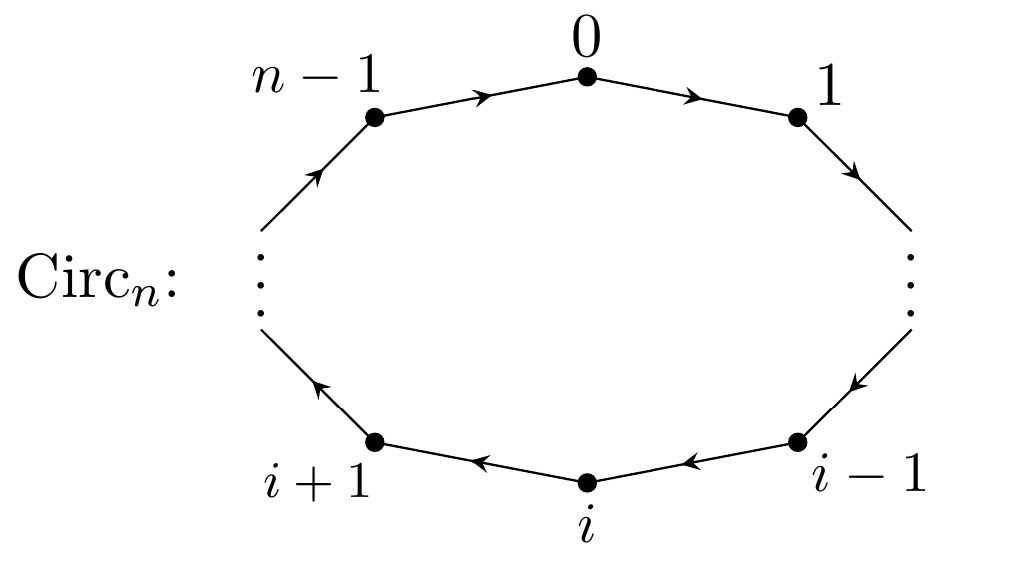
\includegraphics[width=8cm]{assets/circle-graph.png}
        \centering
    \end{figure}
    Trong đó $\Z_n$ là tập các đỉnh, $\{ [i,i+1] \mid i \in \Z_n \}$ là tập các cạnh với định hướng cho bởi $o([i,i+1]) = i$ và $t([i,i+1]) = i + 1$.
\end{define}

\begin{define}[\cite{TreeSerre}]
    Một \textdef{chu trình} độ dài $n$ trong đồ thị bất kì là đồ thị con đẳng cấu với $\Circ_n$.
\end{define}

\begin{define}[\cite{TreeSerre}]
    Một \textdef{cây} là đồ thị liên thông khác rỗng không có chu trình.
\end{define}

% \begin{define}[\cite{TreeSerre}]
%     Cho $G$ là nhóm và $S \subset G$. Ta kí hiệu $\Gamma = \Gamma(G,S)$ là đồ thị có hướng với $G$ là tập đỉnh
% \end{define}
\subsection{Tác động của nhóm lên cây}
\begin{define}[\cite{TreeSerre}]
    Cho $G$ là nhóm và $X$ là đồ thị, một \textdef{tác động} của $G$ lên $X$ là một đồng cấu nhóm $G \rightarrow \Aut(X)$.

    Ta nói $G$ tác động \textdef{tạo cạnh ngược} lên $G$ nếu có phần tử $g \in G$ và cạnh $y \in X$ sao cho $gy = \overline{y}$.

    Nếu $G$ tác động lên $X$ không tạo cạnh ngược thì ta có thể định nghĩa \textdef{đồ thị thương} $G \setminus X$ với tập đỉnh và tập cạnh tương ứng với quỹ đạo dưới tác động $G$ lên $\ver X$ và $\edge X$.

    Nếu $G$ tác động không tạo ra cạnh ngược và không phần tử $g \neq 1$ nào cố định đỉnh của $X$ thì ta nói đây là một \textdef{tác động tự do}.

    Một \textdef{miền cơ bản} của $X$ dưới tác động $G$ là đồ thị con $T$ sao cho cấu xạ cảm sinh $T \rightarrow G \setminus X$ là đẳng cấu. Ta có thể chỉ ra rằng nếu $X$ là cây thì miền cơ bản tồn tại khi và chỉ khi $G \setminus X$ là cây.
\end{define}

\begin{theorem}[\cite{TreeSerre}]\label{thm:bass-serre-fund}
    Cho $G$ là nhóm tác động lên đồ thị $X$, $T$ là cạnh $P \xrightarrow[]{Y} Q$ trong $X$, đồng thời là miền cơ bản của $X$ và kí hiệu $G_P,\ G_Q,\ G_Y$ lần lượt là nhóm con cố định $P$, $Q$ và $Y$. Khi đó $X$ là cây khi và chỉ khi đồng cấu cảm sinh $G_P *_{G_Y} G_Q \rightarrow G$ là đẳng cấu.
\end{theorem}

\subsection{Cây Serre}
Ở phần này ta mặc định $K$ là trường số có định giá rời rạc $v$ và vành định giá $\mathcal{O}$.

\begin{define}[\cite{TreeSerre}]
    Cho $K$ là một trường với vành định giá $\mathcal{O}$. Một \textdef{dàn} trong $K^2$ là một $\mathcal{O}$-môđun tự do có hạng bằng $2$ trong $K^2$.
\end{define}

\begin{remark}[\cite{TreeSerre}]
    Nếu $L$ là dàn trong $K^2$ và $x \in K^*$ thì $L x$ cũng là một dàn, quỹ đạo của $L$ dưới tác động của $K^*$ lên tập các dàn trong $K^2$ được gọi là \textdef{lớp dàn}. Hai dàn $L, L'$ trong $K^2$ được gọi là \textdef{tương đương} nếu chúng cùng nằm trong một lớp dàn, nghĩa là tồn tại phần tử $x \in K^*$ sao cho $L' = L x$, kí hiệu $L \sim L'$.
\end{remark}

\begin{lemma}[\cite{TreeSerre}]
    Nếu $L_0$ và $L_1$ là hai dàn trong $K^2$ thì tồn tại $L_1' \sim L_1$ sao cho $L_1' \subset L_0$.
\end{lemma}

Xét dàn $L_0 = \mathcal{O}v \oplus \mathcal{O}w$ và $L_1$. Từ bổ đề trên, tồn tại $L_1' \sim L_1$ sao cho $L_1' \subset L_0$. Theo Định lí thừa số bất biến của môđun trên vành chính, tồn tại hai số nguyên $a,b$ sao cho
$$
    L_1' = \mathcal{O} \pi^a v \oplus \mathcal{O} \pi^v w,
$$
trong đó $\pi$ là phần tử đồng nhất trong vành định giá $\mathcal{O}$. Khoảng cách giữa hai dàn lúc này được định nghĩa là
$$
    d(L_0, L_1) = |a-b|.
$$
Giá trị $a,b$ ở đây không phụ thuộc vào cách chọn cơ sở cho $\Gamma_0$ và do đó khoảng cách giữa hai dàn được định nghĩa tốt. Hơn nữa nếu ta thay $L_0, L_1$ bởi hai dàn $L_0 x, L_0 y$ $(x,y \in K^*)$ thì hệ số $a,b$ lúc này được thay bằng $a+c, b+c$, trong đó $c = v(y/x)$. Vậy ta có thể nói đến khoảng cách giữa hai lớp dàn tương đương mà không phụ thuộc vào cách chọn phần tử đại diện.

\begin{define_theorem}[\cite{TreeSerre}]
    Đặt $X$ là đồ thị với tập đỉnh là tập các lớp dàn trong $K^2$ và tập cạnh là tập các cặp lớp dàn $(\Lambda,\Lambda')$ sao cho $d(\Lambda,\Lambda') = 1$, ta kí hiệu $\Lambda \Lambda'$ cho một cạnh trong $X$. Lúc này $X$ là cây và $X$ được gọi là \textdef{cây Serre}.
\end{define_theorem}

\startproof Xem \cite[Chương 2, Mục 1.1, Định lí 1]{TreeSerre}.\qed

\subsection{Tác động của $SL_2(K)$ lên cây Serre}

\begin{define}[\cite{TreeSerre}]
    Ta định nghĩa tác động của nhóm $GL_2(K)$ lên dàn $L = \mathcal{O}v \oplus \mathcal{O}w$ cho bởi
    $$
        A(\mathcal{O}v \oplus \mathcal{O}) = \mathcal{O}Av \oplus \mathcal{O}Aw
    $$
    Hơn nữa tác động này bảo toàn khoảng cách giữa hai dàn, do đó $GL_2(K)$ tác động lên cây Serre.
\end{define}

\begin{proposition}[\cite{TreeSerre}]
    Tác động $SL_2(K)$ lên cây Serre giới hạn từ tác động của $GL_2(K)$ không tạo ra cạnh ngược.
\end{proposition}

\begin{theorem}[\cite{TreeSerre}]
    Cho $G$ là nhóm con của $GL_2(K)$. Khi đó nếu bao đóng của $G$ chứa $SL_2(K)$ thì $\Lambda \Lambda'$ là miền cơ bản cho tác động của $G$ lên cây Serre $X$, trong đó $\Lambda \Lambda'$ là một cạnh của $X$. Từ đó dẫn đến
    $$
        G = G_{\Lambda} *_{G_{\Lambda \Lambda'}} G_{\Lambda'},
    $$
    với $G_{\Lambda}, G_{\Lambda'}, G_{\Lambda \Lambda'}$ lần lượt là nhóm con của $G$ cố định $\Lambda, \Lambda'$ và $\Lambda \Lambda'$.
\end{theorem}

\startproof Xem \cite[Chương 2, Mục 1.4, Định lí 2 và Định lí 3]{TreeSerre}.\qed

Bằng cách tính nhóm con cố định đỉnh và cạnh của cây Serre, ta có định lí quan trọng và nổi tiếng sau:

\begin{theorem}[Ihara \cite{TreeSerre}]
    Cho $K$ là trường có định giá rời rạc $v$ với vành định giá $\mathcal{O}$ và phần tử đồng nhất $\pi$. Khi đó
    $$
        SL_2(K) = SL_2(\mathcal{O}) *_\Gamma SL_2(\mathcal{O})
    $$
    % và
    % $$
    %     PSL_2(K) = SL_2(\mathcal{O}) *_{\bar{\Gamma}} PSL_2(\mathcal{O})
    % $$
    với
    $$
        \Gamma = \left\{ \begin{pmatrix}
            * & * \\
            c & *
        \end{pmatrix} \in SL_2(\mathcal{O})\ \middle|\ c \equiv 0\ (\operatorname*{mod}\ \pi) \right\},
    $$
    trong đó hai phép nhúng từ $\Gamma$ vào $SL_2(\mathcal{O})$ cho bởi
    $$
        \begin{pmatrix}
            a & b \\
            c & d
        \end{pmatrix} \mapsto \begin{pmatrix}
            a & b \\
            c & d
        \end{pmatrix}\enskip \text{ và }\enskip \begin{pmatrix}
            a & b \\
            c & d
        \end{pmatrix} \mapsto \begin{pmatrix}
            a         & b\pi         \\
            \pi^{-1}c & \pi^{-1}d\pi
        \end{pmatrix}.
    $$

    % và $\bar{\Gamma} = \Gamma / \{\pm I\}$.
\end{theorem}

\begin{lemma}{\cite{TreeSerre}}
    Nếu $A$ là vành con trù mật trong $K$ thì $SL_2(A)$ trù mật trong $SL_2(K)$.
\end{lemma}
\startproof Bao đóng của $SL_2(A)$ chứa hai nhóm con cộng lần lượt sinh bởi $\begin{pmatrix}
        1 & 1 \\
        0 & 1
    \end{pmatrix}$ và $\begin{pmatrix}
        1 & 0 \\
        1 & 1
    \end{pmatrix}$. Hơn nữa hai ma trận này sinh ra $SL_2(K)$.\qed

\begin{corollary}[\cite{TreeSerre}]\label{cor:amalgam-sl2-1p}
    Với $p$ là số nguyên tố, ta có
    $$
        SL_2(\Z[1/p]) \cong SL_2(\Z) *_{\Gamma_0(p)} SL_2(\Z),
    $$
    trong đó $\Gamma_0(p)$ là nhóm con đồng dư Hecke của $SL_2(\Z)$.
\end{corollary}

\startproof Xem \cite[Chương 2, Mục 1.4, Hệ quả 2]{TreeSerre}.\qed

Từ đó ta có một kết quả tổng quát như sau:

\begin{corollary}[\cite{TreeSerre}]\label{cor:sl2-amalgam}
    Nếu $n$ là số nguyên không có ước nguyên tố $p$ thì khi đó
    $$
        SL_2(\Z[1/pn]) \cong SL_2(\Z[1/n]) *_{\Gamma} SL_2(\Z[1/n]).
    $$
    trong đó
    $$
        \Gamma = \left\{ \begin{pmatrix}
            * & * \\
            c & *
        \end{pmatrix} \in SL_2(\Z[1/n])\ \middle|\ c \equiv 0\ (\operatorname*{mod}\ \pi) \right\}.
    $$
    Vậy nhóm $SL_2(\Z[1/p_1...p_k])$ có thể biểu diễn thành tích amalgam của các nhóm $SL_2(\Z)$ trên các nhóm con đồng dư. Đây là kết quả quan trọng trong công cuộc tính đối đồng điều của nhóm $SL_2(\Z[1/m])$ với $m$ là tích các số nguyên tố phân biệt bất kì.
\end{corollary}